\section{Data understanding} \label{seq:data_understanding}

 In this phase the objective is to consider the available data, understand their properties, check its quality and explore it through statistical methods.

 \subsection{Collect initial data}

The data is collected through a platform called \textit{ballchasing.com} that allows players to download a plugin for the game that will automatically load their replays to to platform.

The replays are then viewable into a web based frontend and is possible to analyze different statistics from the replay. The platform provides also different HTTP API:

\begin{itemize}
    \item \textbf{Get replay}: returns the binary replay file given the ID;
    \item \textbf{Get replay list}: returns a json involving summary of replays (including the ID to get the full replay) given different filters;
    \item \textbf{Get replay statistics}: returns a full detailed statistics of the game for each player given the replay ID;
    \item \textbf{Upload replay} used by the plugin to upload replays;
    \item \textbf{Delete replay}.
\end{itemize}

It is important to clarify that a replay \textbf{is not a video} file as usual, but a large binary file containing various metadata on the match and the players and a table in which are listed all the information necessary to review the match.
Therefore, for each instant \textit{(frame)} of the game, are listed position, direction and velocity vector of each player and the ball, and also other information of the inputs the players is giving (e.g. player is using boost, player is drifting, etc...).

Extracting features from the \textit{raw replays} can be very challenging, and the amount of possible features is quite high. However, the main problem about raw replays is API limitations, as it is possible to download only 200 replays per hour. Instead, we can download the \textit{replay statistics}, as they are very detailed and provide stats about all the players, furthermore the limitation is 2000 per hour.

Thus, in this project, it was used the calculated stats from the APIs. Each downloaded replay is saved in a JSON file. These, are hierarchical files that contain also a lot of metadata and other useless for our task information about the match (e.g. stadium, car personalization of each player etc...). It was discarded this data and take the stats about the six players in the match, which then results in 6 rows for each replay.

Data was collected using \textit{cluster sampling} from the date-hour, thus sampling the start-date, and then getting all the replay in a given range. The date is sampled from a range starting from August 2021 until February 2022, that's because are the dates of the two last \textit{"Seasons"} of Rocket League. At the end of each season there is a soft reset of ranks: the MMR doesn't change but the players have to do again 10 matches where the MMR change at the end of the match is higher.
It was decided to not consider older seasons because the \textit{playstyle} and the distribution of players in Rocket League changes over time.

The sampling was repeated for each rank, changing the hour-range, because for lower ranks, less replays were retrieved; this was an attempt to balance the rank distribution, thus, a sort of stratified sampling.
Anyway, for these ranks, system would return always the same replays, therefore, the process is stopped when the \textit{new\_replays / retrieved\_replays} hit a certain number. The whole process was repeated, adjusting the parameters at each iteration (extension of range for certain ranks, new replay ratio), until \textit{N} replays are retrieved. The target was to have hundred of thousands of replays.

\subsection{Describe data and features}

The resulting dataset counts 404951 rows and 84 features in our data, divided in five categories: Core Stats, Boost Stats, Movement Stats, Poistioning Stats and Demolitions Stats. Let's briefly describe them:

\begin{center}
    \textit{Core Stats}
\end{center}
\begin{itemize}
    \item \textbf{shots}: shots performed;
    \item \textbf{shot}\_against: shots the players undergoes while he is acting as goalkeeper;
    \item \textbf{goals}: goals performed,
    \item \textbf{goals\_against}: goals taken: 
    \item \textbf{saves}: goals saved,
    \item \textbf{assists}: assists performed,
    \item \textbf{score}: score cumulated at the end of the match,
    \item \textbf{mvp}: tells if is the most valuable player in the match,
    \item \textbf{shooting\_percentage}: shots compared to the teams shots
\end{itemize}
\begin{center}
    \textit{Boost Stats}
\end{center}
\begin{itemize}
    \item \textbf{bpm}: boost consumption per minute;
    \item \textbf{bcpm}: boost collected per minute;
    \item \textbf{amount\_collected\_big}: Amount of boost collected with big pads. Boost can be collected through big or mini pads, big ones are at the edges of the playing field, and fulls the boost, mini ones are scattered trough the field and refill only $13 \%$;
    \item \textbf{amount\_collected\_small}: amount of boost collected with mini pads;
    \item \textbf{amount\_stolen\_big}: amount of boost stolen to other players from big pads
    \item \textbf{amount\_stolen\_small}: amount of boost stolen to other players from mini pads
    \item \textbf{count\_collected\_big}: number of big pads taken,
    \item \textbf{count\_collected\_small}: number of mini pads taken,
    \item \textbf{amount\_overfill}: amount of boost extra boost taken from big pads
    \item \textbf{amount\_overfill\_stolen"}: amount of boost extra boost taken from big pads to steal from other players
    \item \textbf{amount\_used\_while\_supersonic"}: amount of boost used while in supersonic speed (useless as it is max speed)
    \item \textbf{time\_zero\_boost}: amount of time player has zero boost in the match;
    \item \textbf{time\_boost\_0\_25}: amount of time player has boost between 0 and 25;
    \item \textbf{time\_boost\_25\_50}: amount of time player has boost between 25 and 50;
    \item \textbf{time\_boost\_50\_75}: amount of time player has boost between 50 and 75;
    \item \textbf{time\_full\_boost}: amount of time player has full boost;
    \item \textbf{percent\_zero\_boost}: percent of time player has zero boost in the match;
    \item \textbf{percent\_boost\_0\_25}: percent of time player has boost between 0 and 25;
    \item \textbf{percent\_boost\_25\_50}: percent of time player has boost between 25 and 50;
    \item \textbf{percent\_boost\_50\_75}: percent of time player has boost between 50 and 75;
    \item \textbf{percent\_full\_boost}: amount of time player has full boost;
    \item \textbf{avg\_amount}: average amount of boost in the match;
\end{itemize}
\begin{center}
    \textit{Movement Stats}
\end{center}
\begin{itemize}
    \item \textbf{avg\_speed};
    \item \textbf{avg\_speed\_percentage}: average speed compare to max speed;
    \item \textbf{total\_distance}: total distance covered in the match
    \item \textbf{time\_slow\_speed}:  time spent moving slower than if you were boosting/dodging, i.e. just using throttle, less than ~1400 uu/s;
    \item \textbf{time\_boost\_speed}: time spent moving at boost speed, e.g. while holding boost/dodging, $~1400+ uu/s$; \\
    \item \textbf{time\_supersonic\_speed}: time spent moving at supersonic speed, $~ 2200+ uu/s$; \\
    \item \textbf{percent\_slow\_speed}: percentage time spent moving slower than if you were boosting/dodging, i.e. just using throttle, less than ~1400 uu/s;
    \item \textbf{percent\_boost\_speed}: percentage of time spent moving at boost speed, e.g. while holding boost/dodging, $~1400+ uu/s$; \\
    \item \textbf{percent\_supersonic\_speed}: percentage of time spent moving at supersonic speed, $~ 2200+ uu/s$; \\
    \item \textbf{time\_ground}: amount of time spent on the ground
    \item \textbf{time\_low\_air}: amount of time spent in air but at low altitude w.r.t. the field
    \item \textbf{time\_high\_air}: amount of time spent in air but at high altitude w.r.t. the field
    \item \textbf{percent\_ground}: percentage of time spent on the ground
    \item \textbf{percent\_low\_air}: percentage of time spent in air but at low altitude w.r.t. the field
    \item \textbf{percent\_high\_air}: percentage of time spent in air but at high altitude w.r.t. the field
    \item \textbf{time\_powerslide}: amount of time spent powersliding
    \item \textbf{count\_powerslide}: number of times player uses powerslide;
    \item \textbf{avg\_powerslide\_duration};
\end{itemize}
\begin{center}
    \textit{Positioning Stats}
\end{center}
\begin{itemize}
    \item \textbf{avg\_distance\_to\_ball};
    \item \textbf{avg\_distance\_to\_ball\_possession}: Average distance to the ball while possessing the ball
    \item \textbf{avg\_distance\_to\_ball\_no\_possession}: Average distance to the ball while not possessing the ball
    \item \textbf{avg\_distance\_to\_mates};
    \item \textbf{time\_defensive\_third}: amount of time player is in 1/3 of the field where his net is;
    \item \textbf{time\_neutral\_third}: amount of time player is in the neutral third;
    \item \textbf{time\_offensive\_third}: amount of time player is in 1/3 of the field where the opponent net is;
    \item \textbf{percent\_defensive\_third}: percentage of time player is in 1/3 of the field where his net is;
    \item \textbf{percent\_neutral\_third}: percentage of time player is in the neutral third;
    \item \textbf{percent\_offensive\_third}: percentage of time player is in 1/3 of the field where the opponent net is;
    \item \textbf{time\_offensive\_half}: amount of time player is in opponent half; \\
    \item \textbf{time\_defensive\_half}: amount of time player is in his team half; \\
    \item \textbf{percent\_offensive\_half}: percentage of time player is in opponent half; \\
    \item \textbf{percent\_defensive\_half}: percentage of time player is in his team half; \\
    \item \textbf{time\_behind\_ball}: amount of time the player is closer to its net than the ball; \\
    \item \textbf{time\_infront\_ball}: amount of time the player is closer to the opponent net than the ball; \\
    \item \textbf{percent\_behind\_ball}: percentage of time the player is closer to its net than the ball; \\
    \item \textbf{percent\_infront\_ball}: percentage of time the player is closer to the opponent net than the ball; \\
    \item \textbf{time\_farthest\_from\_ball}: amount of time he is the player farthest from ball; \\
    \item \textbf{time\_closest\_from\_ball}: amount of time he is the player closest from ball; \\
    \item \textbf{percent\_farthest\_from\_ball}: percentage of time he is the player farthest from ball; \\
    \item \textbf{percent\_closest\_from\_ball}: percentage of time he is the player closest from ball; \\
    \item \textbf{time\_most\_back}: amount of time he was the last defender of its team; \\
    \item \textbf{time\_most\_forward}: amount of time he was the first attacker of its team; \\
    \item \textbf{percentage\_most\_back}: amount of time he was the last defender of its team; \\
    \item \textbf{percentage\_most\_forward}: amount of time he was the first attacker of its team; \\
    \item \textbf{goals\_against\_while\_last\_defender};
\end{itemize}
\begin{center}
    \textit{Demolitions Stats}
\end{center}
\begin{itemize}
    \item \textbf{inflicted}: demolitions inflicted to opponent players;
    \item \textbf{taken}: demolitions taken by opponent players.
\end{itemize}

We can right away notice that there are a lot of features correlated, all the time / percent features are a repetition and we could keep only one among the twos.

Among these we can distinguish \textbf{categorical} and \textbf{numeric features} (\reftab{tab:catdiscr}):

\pagebreak
\begin{longtable}{p{.50\textwidth} p{.50\textwidth}} 
\toprule
\multicolumn{2}{c}{\textbf{Categorical}}                                        \\
\midrule
mvp                                     &                                         \\
 & \\
\toprule
\multicolumn{2}{c}{\textbf{Dicsrete}} \\
\midrule
saves                                   & goals\_against\_while\_last\_defender   \\
assists                                 & shots                                   \\
goals                                   & inflicted                               \\
taken                                   &                                         \\
& \\
\toprule
\multicolumn{2}{c}{\textbf{Continuous}}                                           \\
\midrule
percent\_closest\_to\_ball              & time\_offensive\_half                   \\
avg\_speed\_percentage                  & percent\_boost\_25\_50                  \\
amount\_collected\_small                & amount\_collected                       \\
bcpm                                    & percent\_farthest\_from\_ball           \\
avg\_distance\_to\_mates                & percent\_high\_air                      \\
percent\_slow\_speed                    & time\_behind\_ball                      \\
time\_supersonic\_speed                 & percent\_offensive\_half                \\
count\_powerslide                       & time\_zero\_boost                       \\
percent\_ground                         & shooting\_percentage                    \\
count\_stolen\_small                    & amount\_stolen\_small                   \\
avg\_speed                              & percent\_behind\_ball                   \\
percent\_zero\_boost                    & avg\_powerslide\_duration               \\
time\_boost\_50\_75                     & amount\_stolen\_big                     \\
goals\_against                          & percent\_defensive\_half                \\
time\_most\_back                        & percent\_defensive\_third               \\
time\_farthest\_from\_ball              & percent\_low\_air                       \\
count\_collected\_small                 & time\_full\_boost                       \\
time\_offensive\_third                  & time\_defensive\_half                   \\
amount\_collected\_big                  & count\_collected\_big                   \\
time\_high\_air                         & amount\_stolen                          \\
time\_defensive\_third                  & shots\_against                          \\
avg\_amount                             & time\_neutral\_third                    \\
time\_slow\_speed                       & percent\_most\_forward                  \\
percent\_neutral\_third                 & avg\_distance\_to\_ball\_no\_possession \\
time\_closest\_to\_ball                 & total\_distance                         \\
percent\_boost\_0\_25                   & time\_low\_air                          \\
time\_infront\_ball                     & avg\_distance\_to\_ball                 \\
score                                   & time\_boost\_25\_50                     \\
time\_boost\_0\_25                      & time\_boost\_speed                      \\
amount\_overfill                        & time\_boost\_75\_100                    \\
bpm                                     & time\_ground                            \\
avg\_distance\_to\_ball\_possession     & time\_powerslide                        \\
percent\_boost\_50\_75                  & percent\_boost\_75\_100                 \\
percent\_most\_back                     & percent\_boost\_speed                   \\
count\_stolen\_big                      & amount\_used\_while\_supersonic         \\
percent\_offensive\_third               & percent\_supersonic\_speed              \\
amount\_overfill\_stolen                & time\_most\_forward                     \\
percent\_full\_boost                    & percent\_infront\_ball                  \\
\bottomrule
\caption{Categorical and discrete feature disctinction}
\label{tab:catdiscr}             
\end{longtable}

\subsection{Verify data quality}

All of the data is automatically generated and collected, thus, is not subject to human errors.
We cannot ensure that data is \textit{accurate}, so that stored value is the actual value, but, a simple consistency check can but run.
Most of the features are percentages, counts and times, therefore they should be greater than 0; in particular, percentages should be also lower than 100. All the rows passed this check.

Data is \textbf{incomplete}. There where a bunch of missing data in some dozen of rows in columns:\textit{percent\_closest\_to\_ball} \textit{percent\_farthest\_from\_ball}, \textit{percent\_most\_forward}, \\ \textit{avg\_distance\_to\_mates}, \textit{time\_most\_back} and also in the target row, \textit{tier}. \\
Missing values in this case are originated from leaving the match before the end, causing errors in the calculation of the metrics. We can notice that most of the missing values are in Bronze ranks, because they tend to care less about their rank and the game in general (leaving a ranked match will count as a loss and will ban you for short period from the ranked matches).

Data is \textbf{consistent}: time measurements are given in seconds, distances in \textit{unreal units (= centimeters)} speeds in \textit{unreal units per second}; then we have counts and percentages.

Data is \textbf{up-to date}: data refers to a single match, and is calculated from the replay file. After the end, it cannot be updated so can't be outdated.

\subsection{Clean data}

In order to calculate summary statistics on our data we need to get rid of missing values and errors in our data.
In this case the most appropriate solution is also the most simple, as the number of rows containing missing values are 199, thus, removing this rows from the dataset.

\subsection{Data exploration}

Let's see some statistics from our data:

\begin{figure}[H]
    \resizebox{1.1\linewidth}{!}{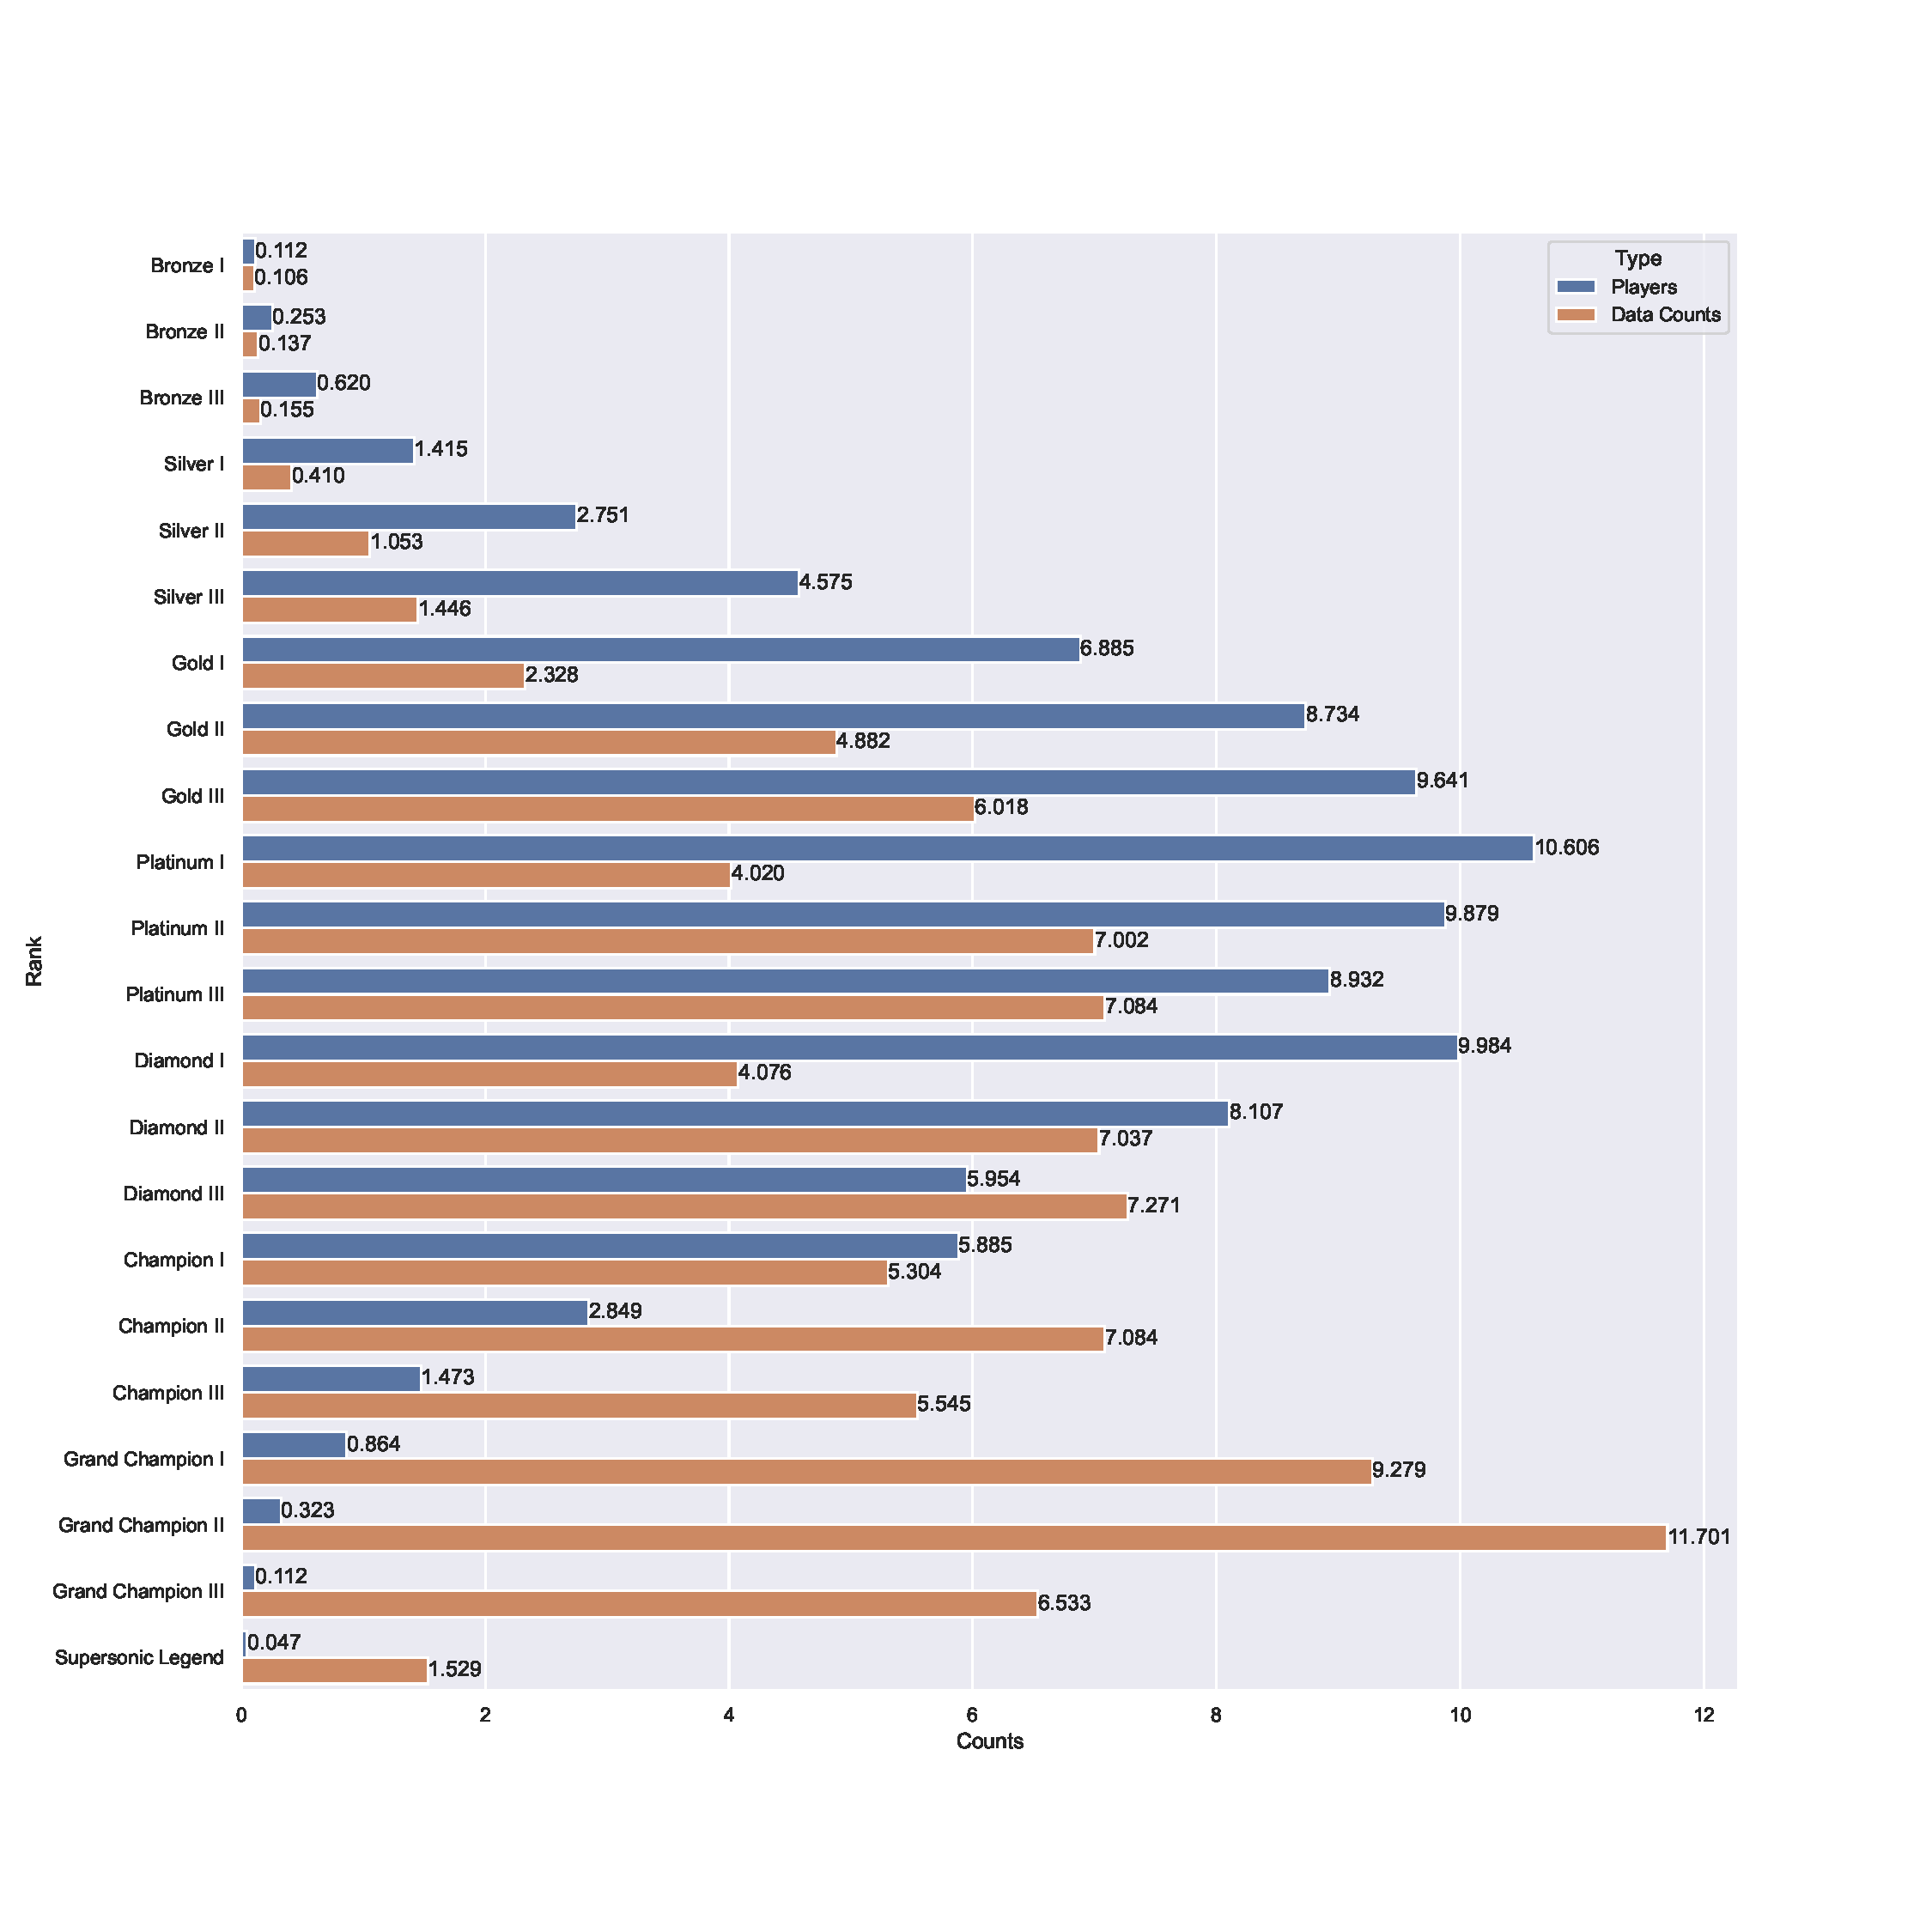
\includegraphics{res/imgs/tiers.pdf}}
    \label{fig:rank_distr}
    \caption{Distribution of players ranks (blue) vs. distribution of ranks in data (orange)}
\end{figure}

We can notice that the the bronze class had very few examples. This has two main reasons, the first one is that there are actually very few players in bronze, it's very difficult to get there basing on how ranking system works. The second reason is that players in bronze are casuals players that even don't know about the plugin necessary to upload replays. We can see the distribution of ranks for the current season (Season 5) in \reffig{fig:rank_distr} (orange). In the same figure we can see in blue the actual distribution of players, that is more or less normally distributed and centered. The data distribution is instead shifted to the right; as we said, skilled players tends to use and know about the plugin.

Histograms and distribution plots have been made for all the features. However, distributions haven't shown no surprises and were quite expected; unless for a light skewness of some (e.g. percent\_full\_boost, time\_high\_air). An exception, is amount stolen big, that shows a mixture distribution with seven gaussians.
In the following features, some of the mentioned plots are shown \reffig{fig:cat_features}:

\begin{figure}[H]
    \centering
    \begin{tabular}{cc}
        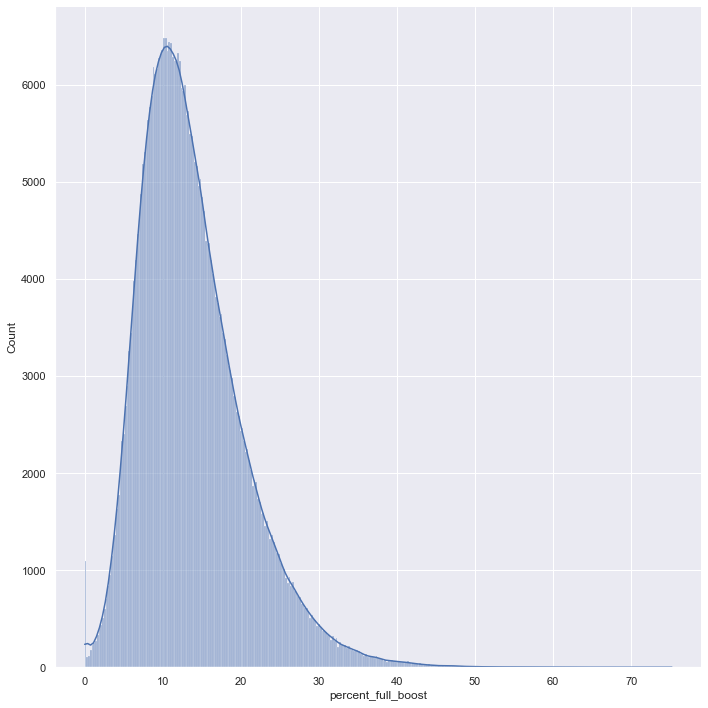
\includegraphics[width=0.5\linewidth]{res/imgs/plots/perrcent_boost.png} &
        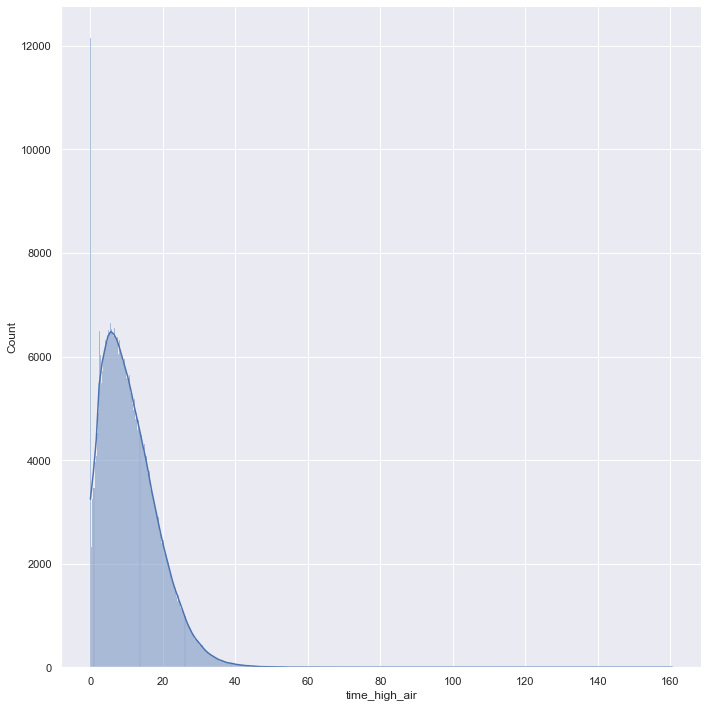
\includegraphics[width=0.5\linewidth]{res/imgs/plots/time.png} \\
        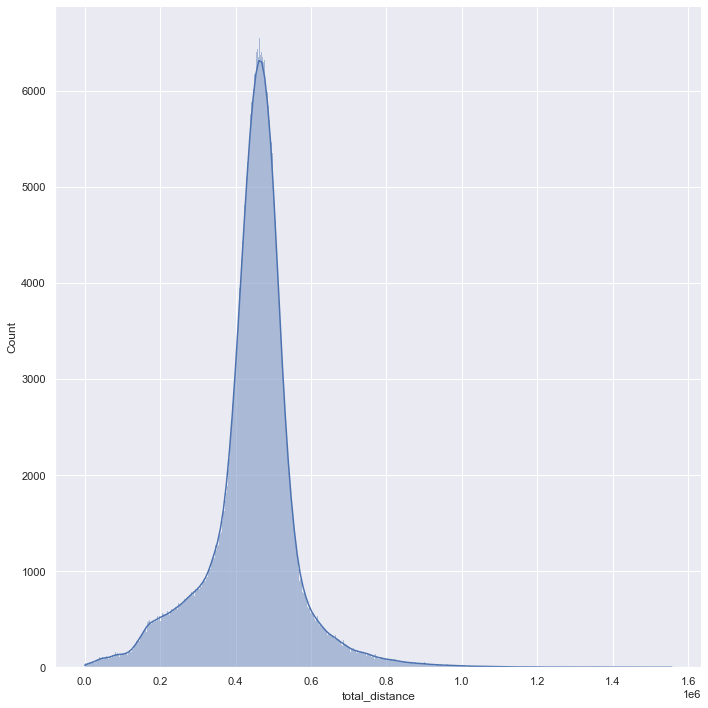
\includegraphics[width=0.5\linewidth]{res/imgs/plots/distance.png} &
        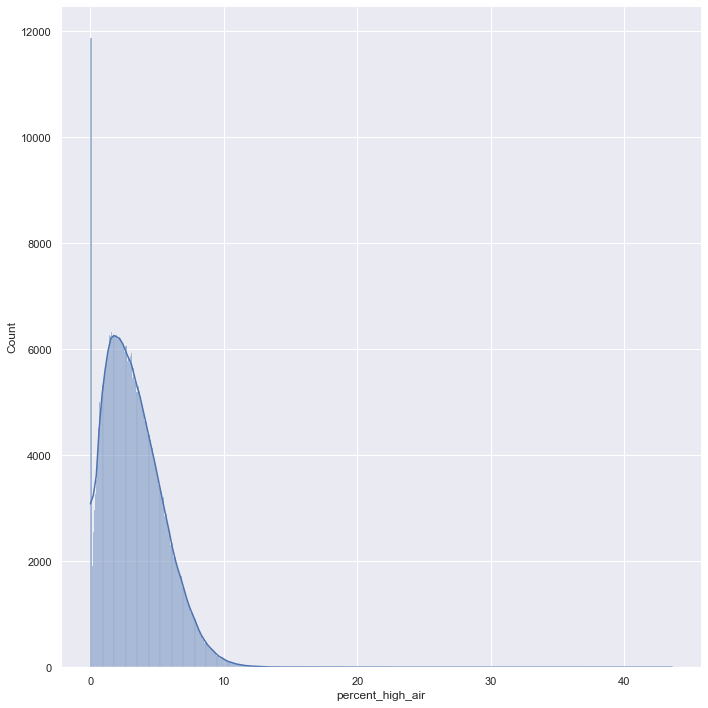
\includegraphics[width=0.5\linewidth]{res/imgs/plots/high_air.png} \\
    \end{tabular}
    \caption{Distribution plot of some continuous features}
    \label{fig:cat_features}
\end{figure}

\begin{figure}[H]
    \centering
    \begin{tabular}{cc}
        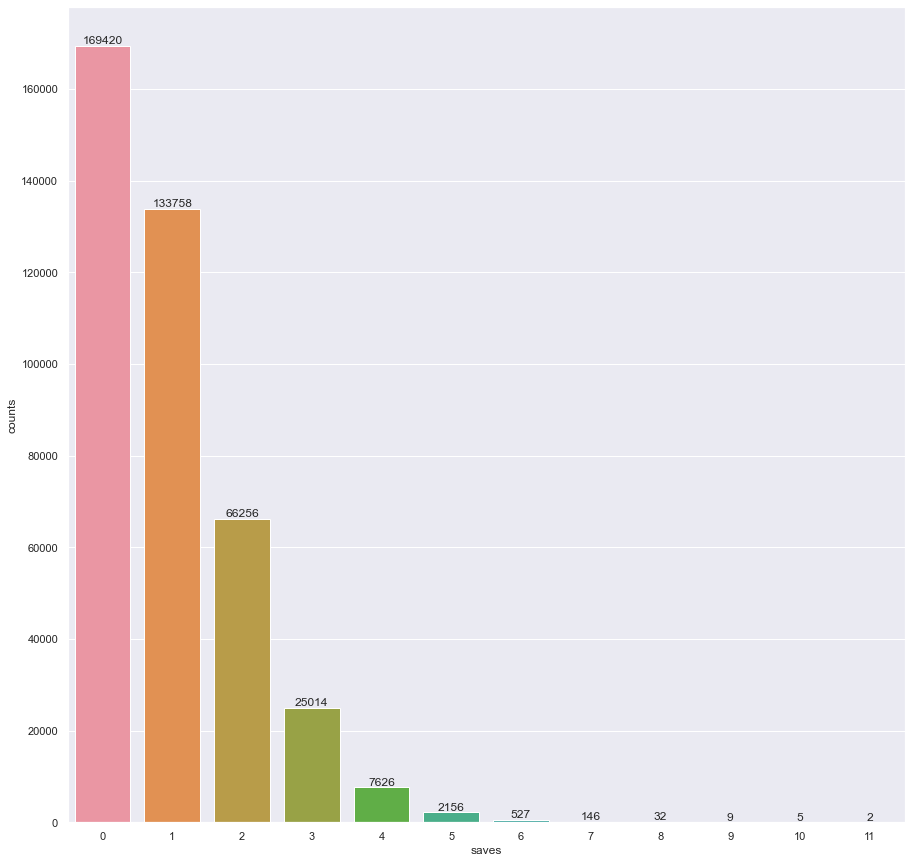
\includegraphics[width=0.5\linewidth]{res/imgs/plots/saves.png} &
        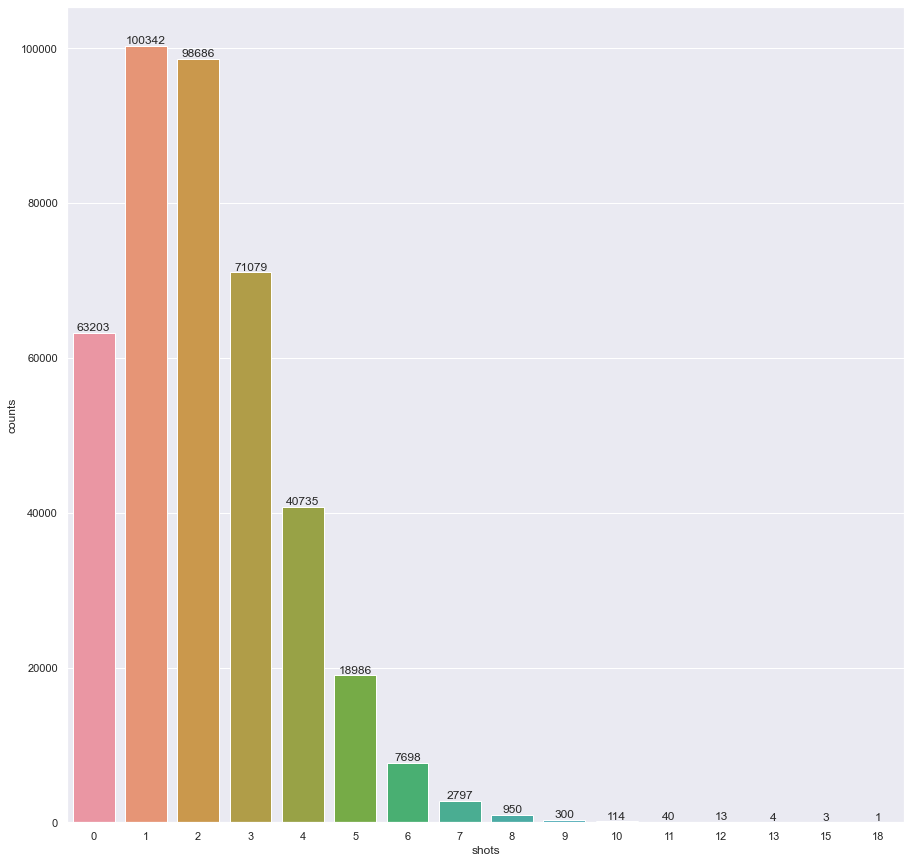
\includegraphics[width=0.5\linewidth]{res/imgs/plots/shots.png} \\
        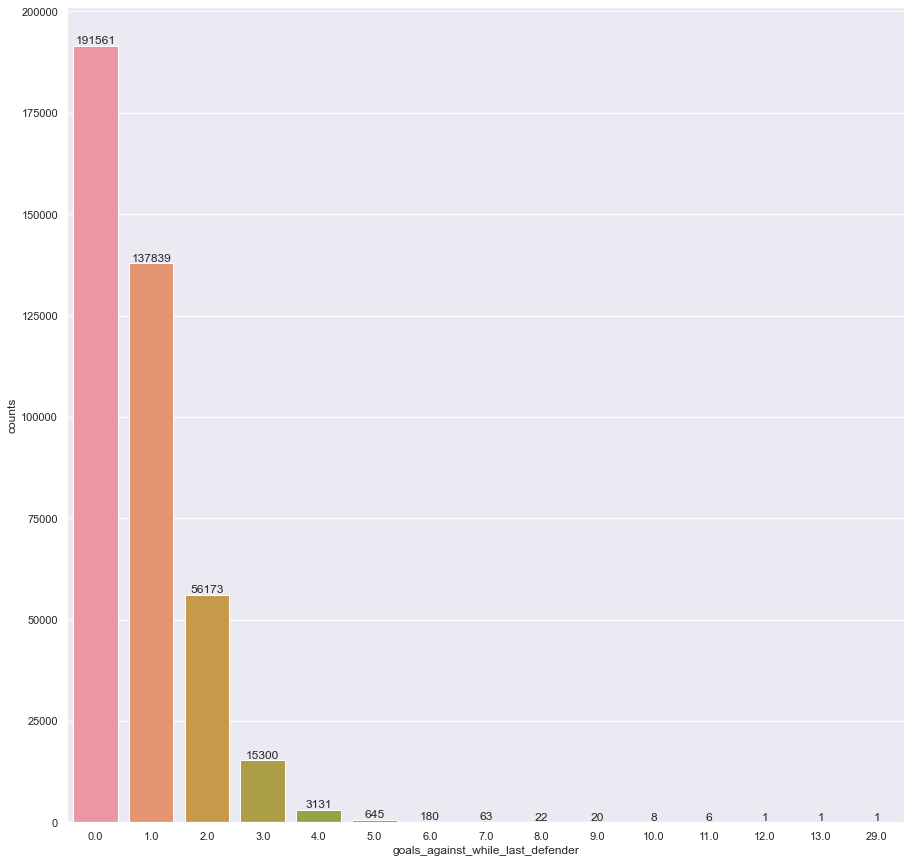
\includegraphics[width=0.5\linewidth]{res/imgs/plots/goal_against.png} &
        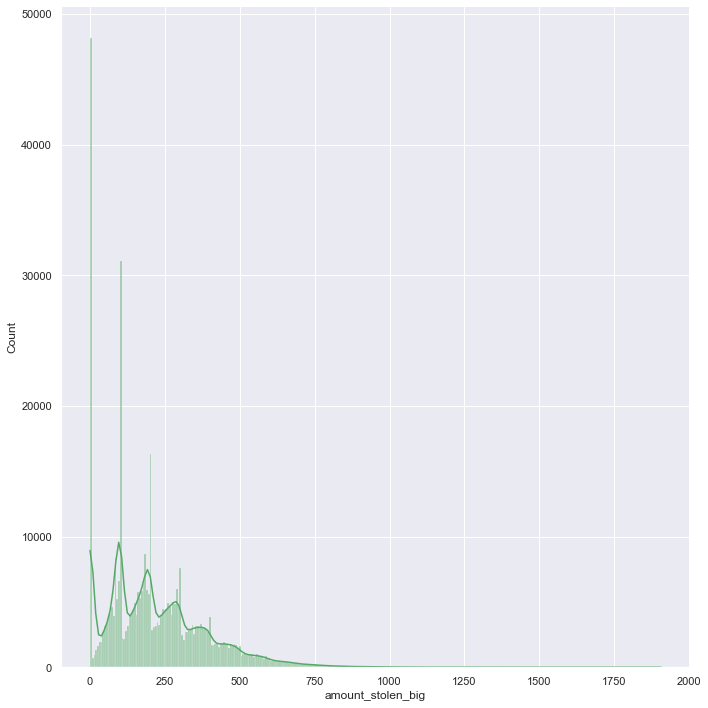
\includegraphics[width=0.5\linewidth]{res/imgs/plots/stolen_big.png} \\
        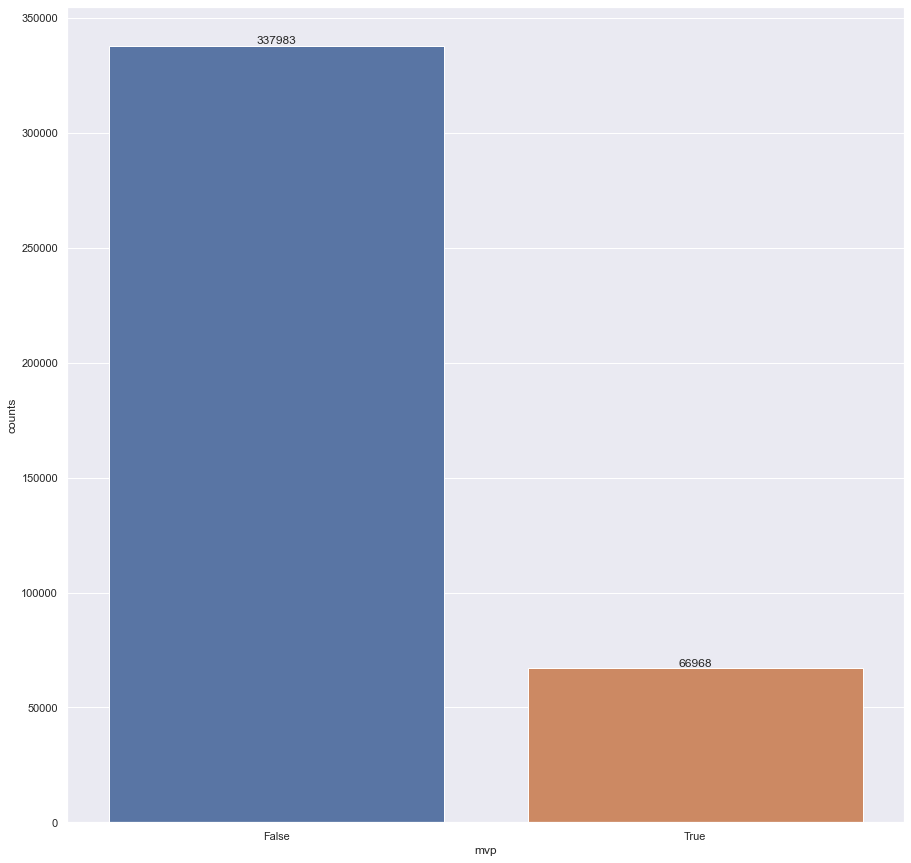
\includegraphics[width=0.5\linewidth]{res/imgs/plots/mvp.png} &
        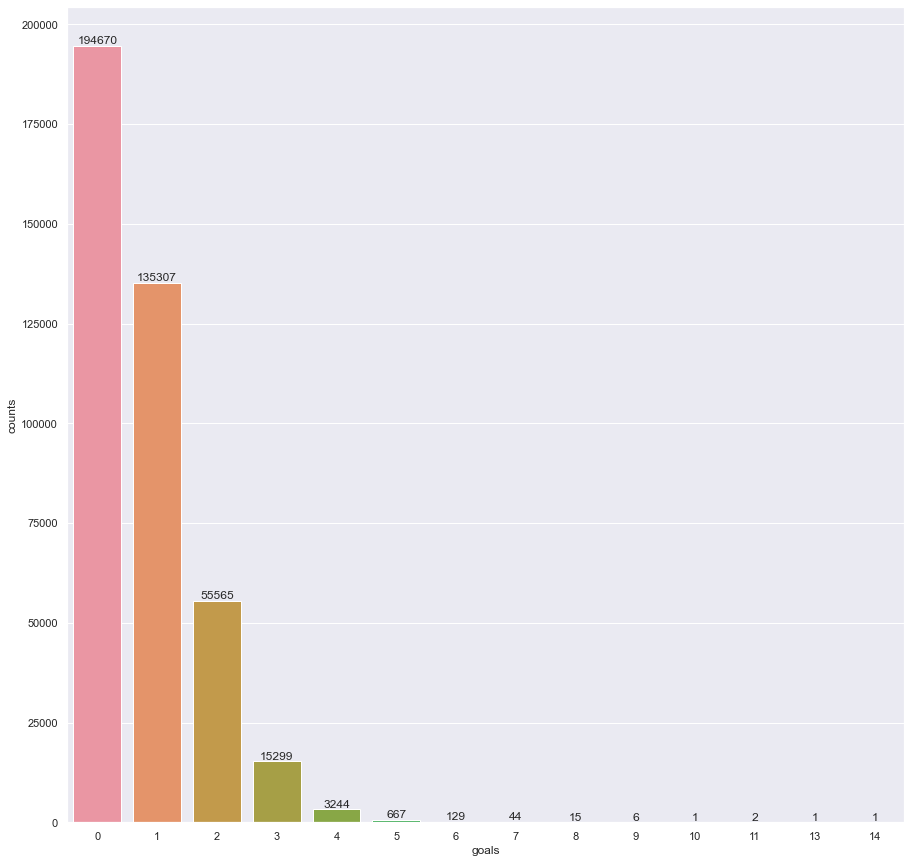
\includegraphics[width=0.5\linewidth]{res/imgs/plots/goals.png} \\
    \end{tabular}
    \caption{Histogram of some discrete features}
    \label{fig:cat_features}
\end{figure}

\section{Data preparation}

Data selection was automatically performed during the collection of the dataset. As already said, replays are randomly sampled between two dates representing two Rocket League seasons.

For feature selection the situation is different, the number of features is quite high and we can early see that some of the are correlated, thus we plot a correlation matrix \reftab{fig:corr_matrix}:

\begin{figure}[H]
    \resizebox{1.1\linewidth}{!}{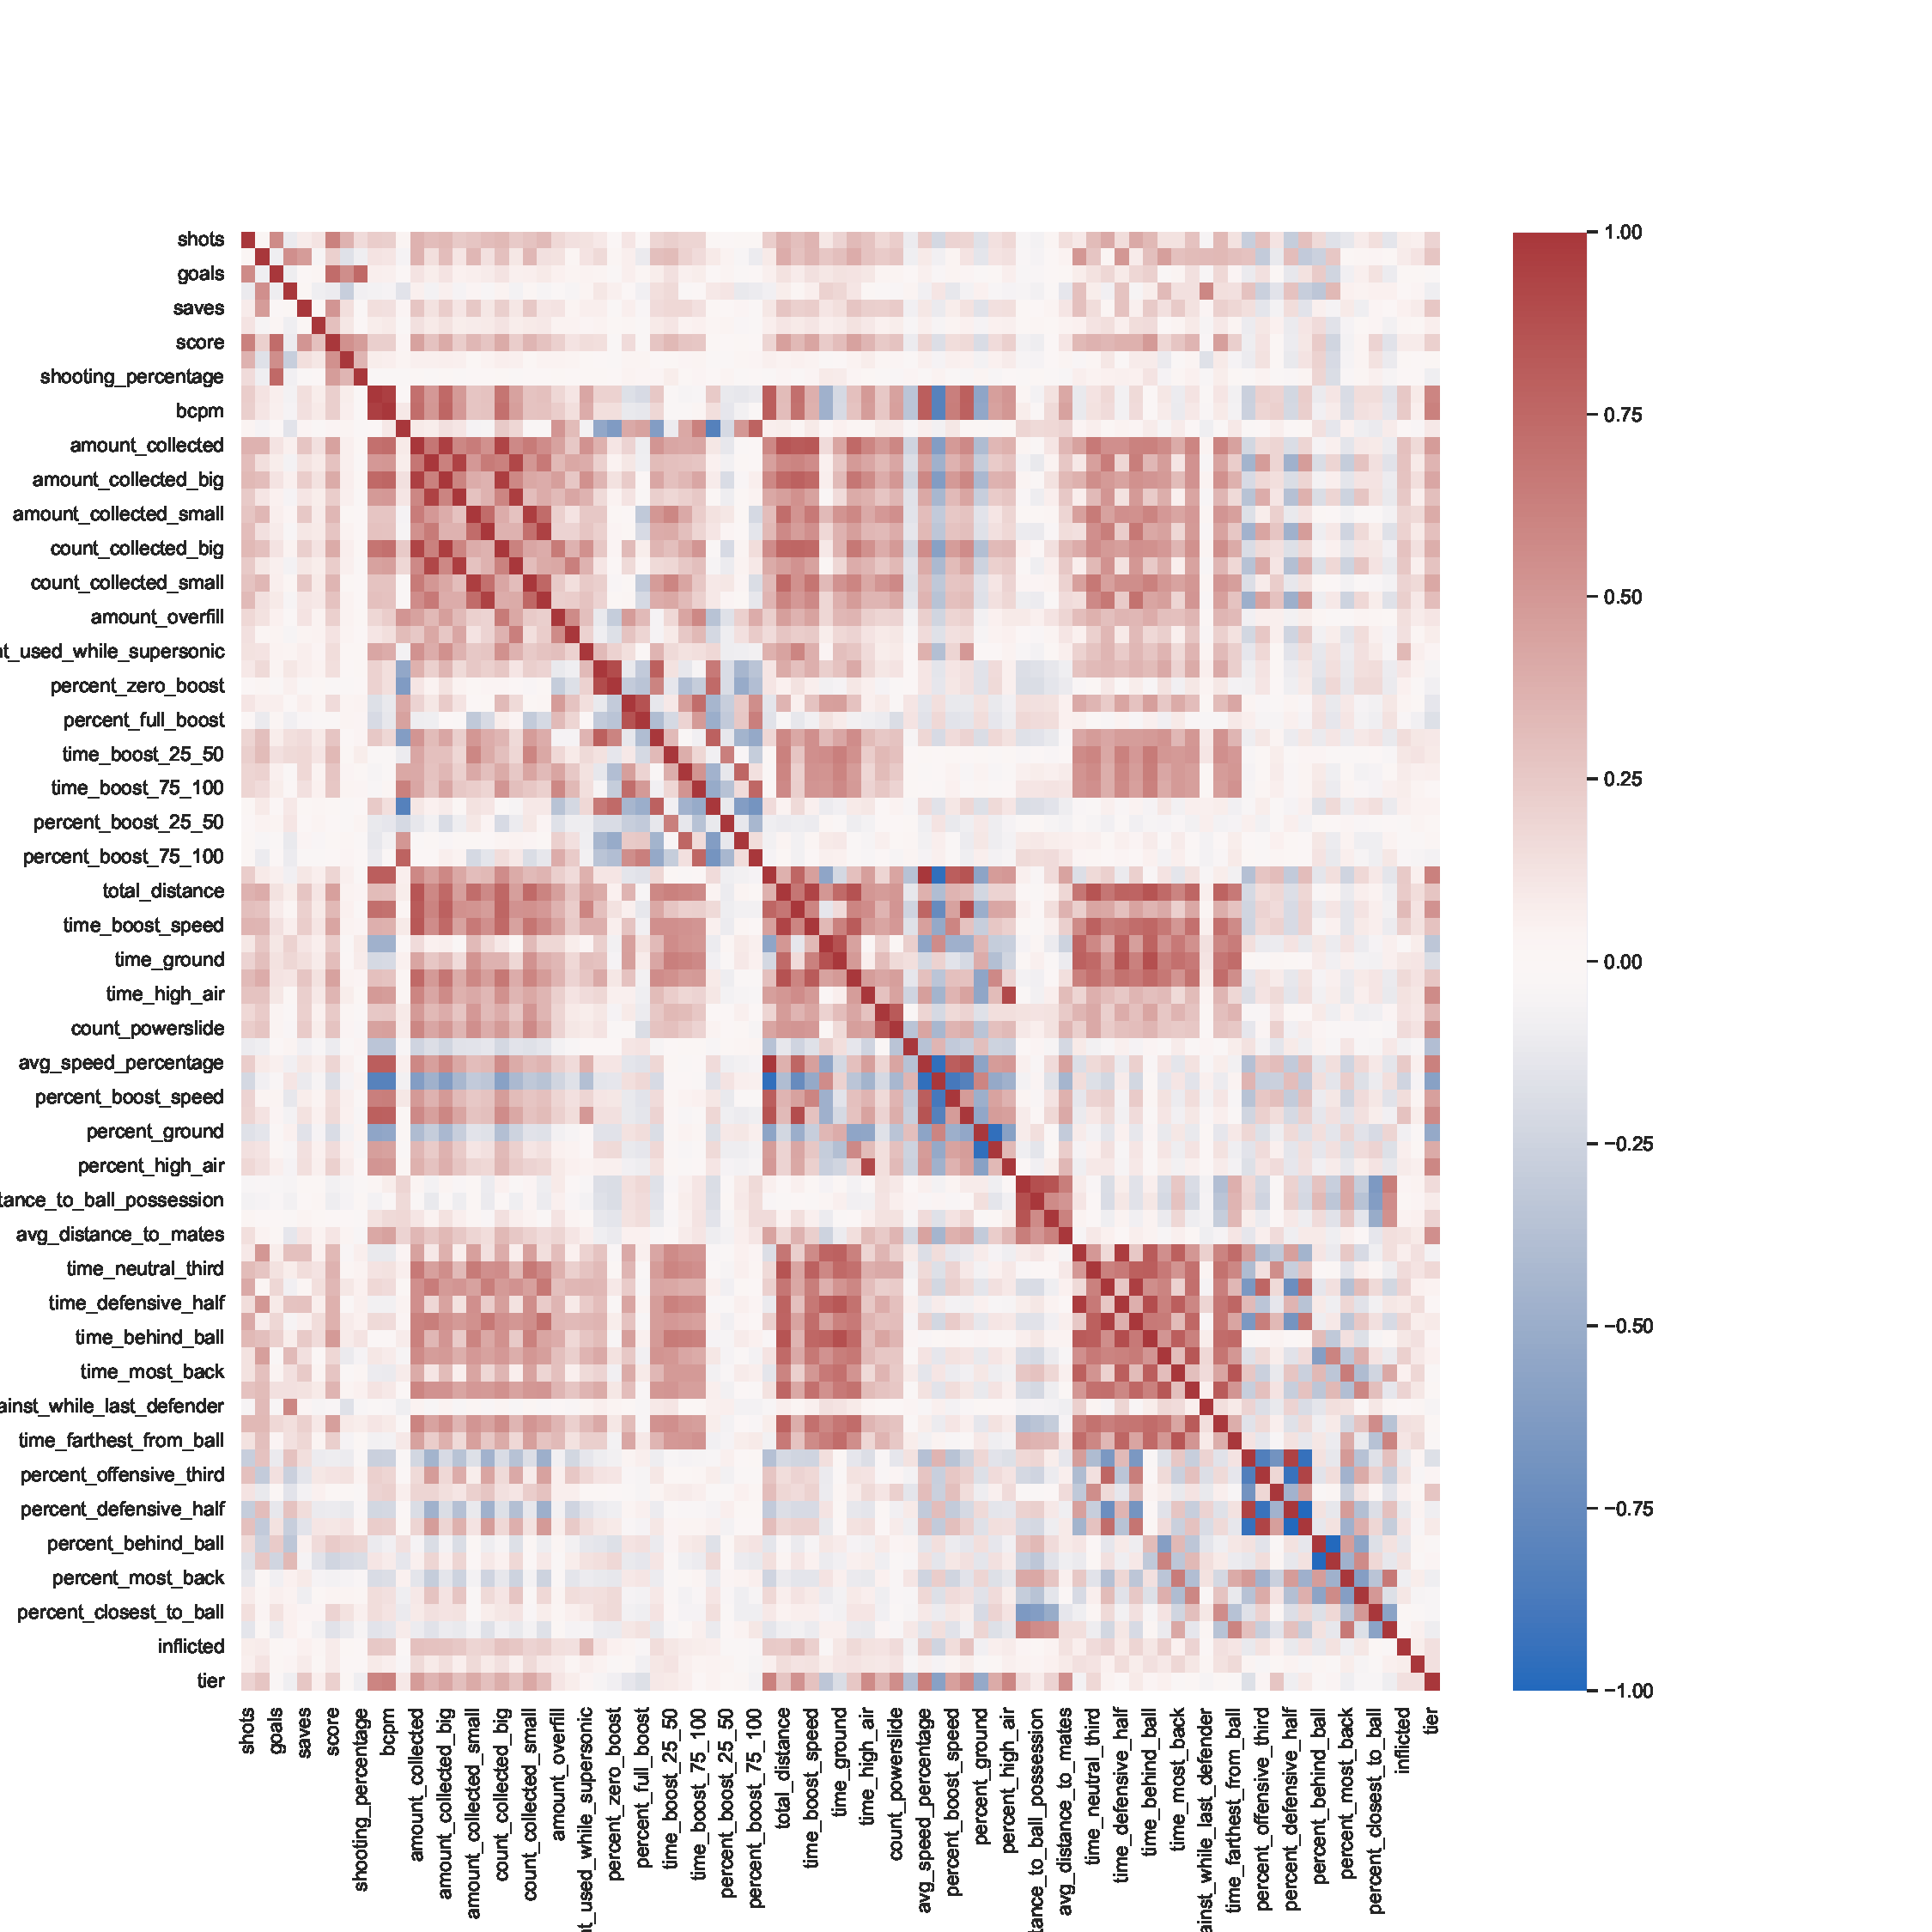
\includegraphics{res/imgs/correlations.pdf}}
    \label{fig:corr_matrix}
    \caption{Features correlation matrix}
\end{figure}

\begin{table}[]
    \scriptsize
    \center
    \begin{tabular}{|l|l|l|}
    \hline
    \textbf{Deleted feature}   & \textbf{Correlated feature}                         & \textbf{Motivation}                                                                                                        \\ \hline
    time\_offensive\_half      & time\_offensive\_third                              & trivial                                                                                                                    \\ \hline
    time\_defensive\_half      & time\_defensive\_third                              & trivial                                                                                                                    \\ \hline
    time\_behind\_ball         & time\_infront\_ball                                 & trivial                                                                                                                    \\ \hline
    time\_infront\_ball        & percent\_infront\_ball                              & trivial                                                                                                                    \\ \hline
    time\_ground               & time\_low\_air, time\_high\_air                     & sum up to 1                                                                                                                \\ \hline
    time\_slow\_speed          & time\_boost\_speed, time\_supersonic\_speed         & sum up to 1                                                                                                                \\ \hline
    time\_most\_back           & time\_most\_forward                                 & trivial                                                                                                                    \\ \hline
    time\_most\_forward        & time\_infront\_ball                                 & \begin{tabular}[c]{@{}l@{}}player whos most forward is\\ usually infront of the ball\end{tabular}                          \\ \hline   
    time\_boost\_speed         & percent\_boost\_speed                               & trivial                                                                                                                    \\ \hline
    time\_closter\_to\_ball    & percent\_closter\_to\_ball                          & trivial                                                                                                                    \\ \hline
    percent\_defensive\_half   & percent\_offensive\_half                            & trivial                                                                                                                    \\ \hline
    percent\_behind\_ball      & percent\_infront\_ball                              & trivial                                                                                                                    \\ \hline
    avg\_speed                 & percent\_slow\_speed                                & trivial                                                                                                                    \\ \hline
    percent\_ground            & percent\_low\_air, percent\_high\_air               & sum up to 1                                                                                                                \\ \hline
    time\_farthest\_from\_ball & time\_defensive\_third                              & \begin{tabular}[c]{@{}l@{}}defender is most of the\\ time farthest from ball\end{tabular}                                  \\ \hline
    percent\_boost\_75\_100    & percent\_boost\_X\_Y                                & sum up to 1                                                                                                                \\ \hline
    time\_boost\_0\_25         & percent\_boost\_0\_25                               & trivial                                                                                                                    \\ \hline
    time\_boost\_25\_50        & percent\_boost\_25\_50                              & trivial                                                                                                                    \\ \hline
    time\_boost\_50\_75        & percent\_boost\_50\_75                              & trivial                                                                                                                    \\ \hline
    time\_boost\_75\_100       & percent\_boost\_75\_100                             & trivial                                                                                                                    \\ \hline
    time\_defensive\_third     & percent\_defensive\_third                           & trivial                                                                                                                    \\ \hline
    time\_neutral\_third       & percent\_neutral\_third                             & trivial                                                                                                                    \\ \hline
    time\_offensive\_third     & percent\_offensive\_third                           & trivial                                                                                                                    \\ \hline
    percent\_offensive\_half   & percent\_offensive\_third                           & Third is more specific than half                                                                                           \\ \hline
    percent\_defensive\_half   & percent\_offensive\_third                           & Third is more specific than half                                                                                           \\ \hline
    percent\_defensive\_third  & percent\_offensive\_third   percent\_neutral\_third & sum up to 1                                                                                                                \\ \hline
    percent\_slow\_speed       & percent\_boost\_speed                               & sum up to 1                                                                                                                \\ \hline
    avg\_amount                & percent\_boost                                      & trivial                                                                                                                    \\ \hline
    avg\_speed\_percentage     & avg\_speed                                          & trivial                                                                                                                    \\ \hline
    time\_defensive\_half      & percent\_defensive\_half                            & trivial                                                                                                                    \\ \hline
    time\_offensive\_half      & percent\_offensive\_half                            & trivial                                                                                                                    \\ \hline
    count\_collected\_big      & amount\_collected\_big                              & trivial                                                                                                                    \\ \hline
    count\_collected\_small    & amount\_collected\_small                            & trivial                                                                                                                    \\ \hline
    count\_stolen\_big         & amount\_stolen\_big                                 & trivial                                                                                                                    \\ \hline
    count\_stolen\_small       & amount\_stolen\_small                               & trivial                                                                                                                    \\ \hline
    time\_low\_air             & time\_boost\_speed                                  & \begin{tabular}[c]{@{}l@{}}When jumping in low air\\ players usually use boost\end{tabular}                                \\ \hline
    time\_high\_air            & percent\_high\_air                                  & trivial                                                                                                                    \\ \hline
    time\_supersonic\_speed    & percent\_supersonic\_speed                          & trivial                                                                                                                    \\ \hline
    time\_zero\_boost          & percent\_zero\_boost                                & trivial                                                                                                                    \\ \hline
    time\_full\_boost          & percent\_full\_boost                                & trivial                                                                                                                    \\ \hline
    amount\_stolen             & amount\_stolen\_big                                 & trivial                                                                                                                    \\ \hline
    amount\_collected          & amount\_collected\_big                              & trivial                                                                                                                    \\ \hline
    avg\_distance\_to\_ball    & avg\_distance\_to\_ball\_possession                 & \begin{tabular}[c]{@{}l@{}}avg\_distance\_to\_ball is more general\\ than avg\_distance\_to\_ball\_possession\end{tabular} \\ \hline
    total\_distance            & time\_boost\_speed                                  & The fast player is the more it travels                                                                                     \\ \hline
    time\_powerslide           & count\_powerslide                                   & trivial                                                                                                                    \\ \hline
    bcpm                       & bpm                                                 & \begin{tabular}[c]{@{}l@{}}Boost consumption is directly\\ connected to boost usage\end{tabular}                           \\ \hline
    \end{tabular}
    \caption{List of deleted features and the correlated ones}
    \label{tab:corr_features}
    \end{table}

By this selection we removed 42 features, thus, halving the dataset vertically. The adopted criterion is based on logical correlation, thus, by inspecting correlations, the removed features are the ones where we can find a motivation for the correlation, otherwise the correlation can be spurious.

In order to further reduce the dimensionality of the dataset another a test have been ran: the information gain test, results are shown in \reffig{fig:ig}:

\begin{figure}[H]
    \resizebox{1.1\linewidth}{!}{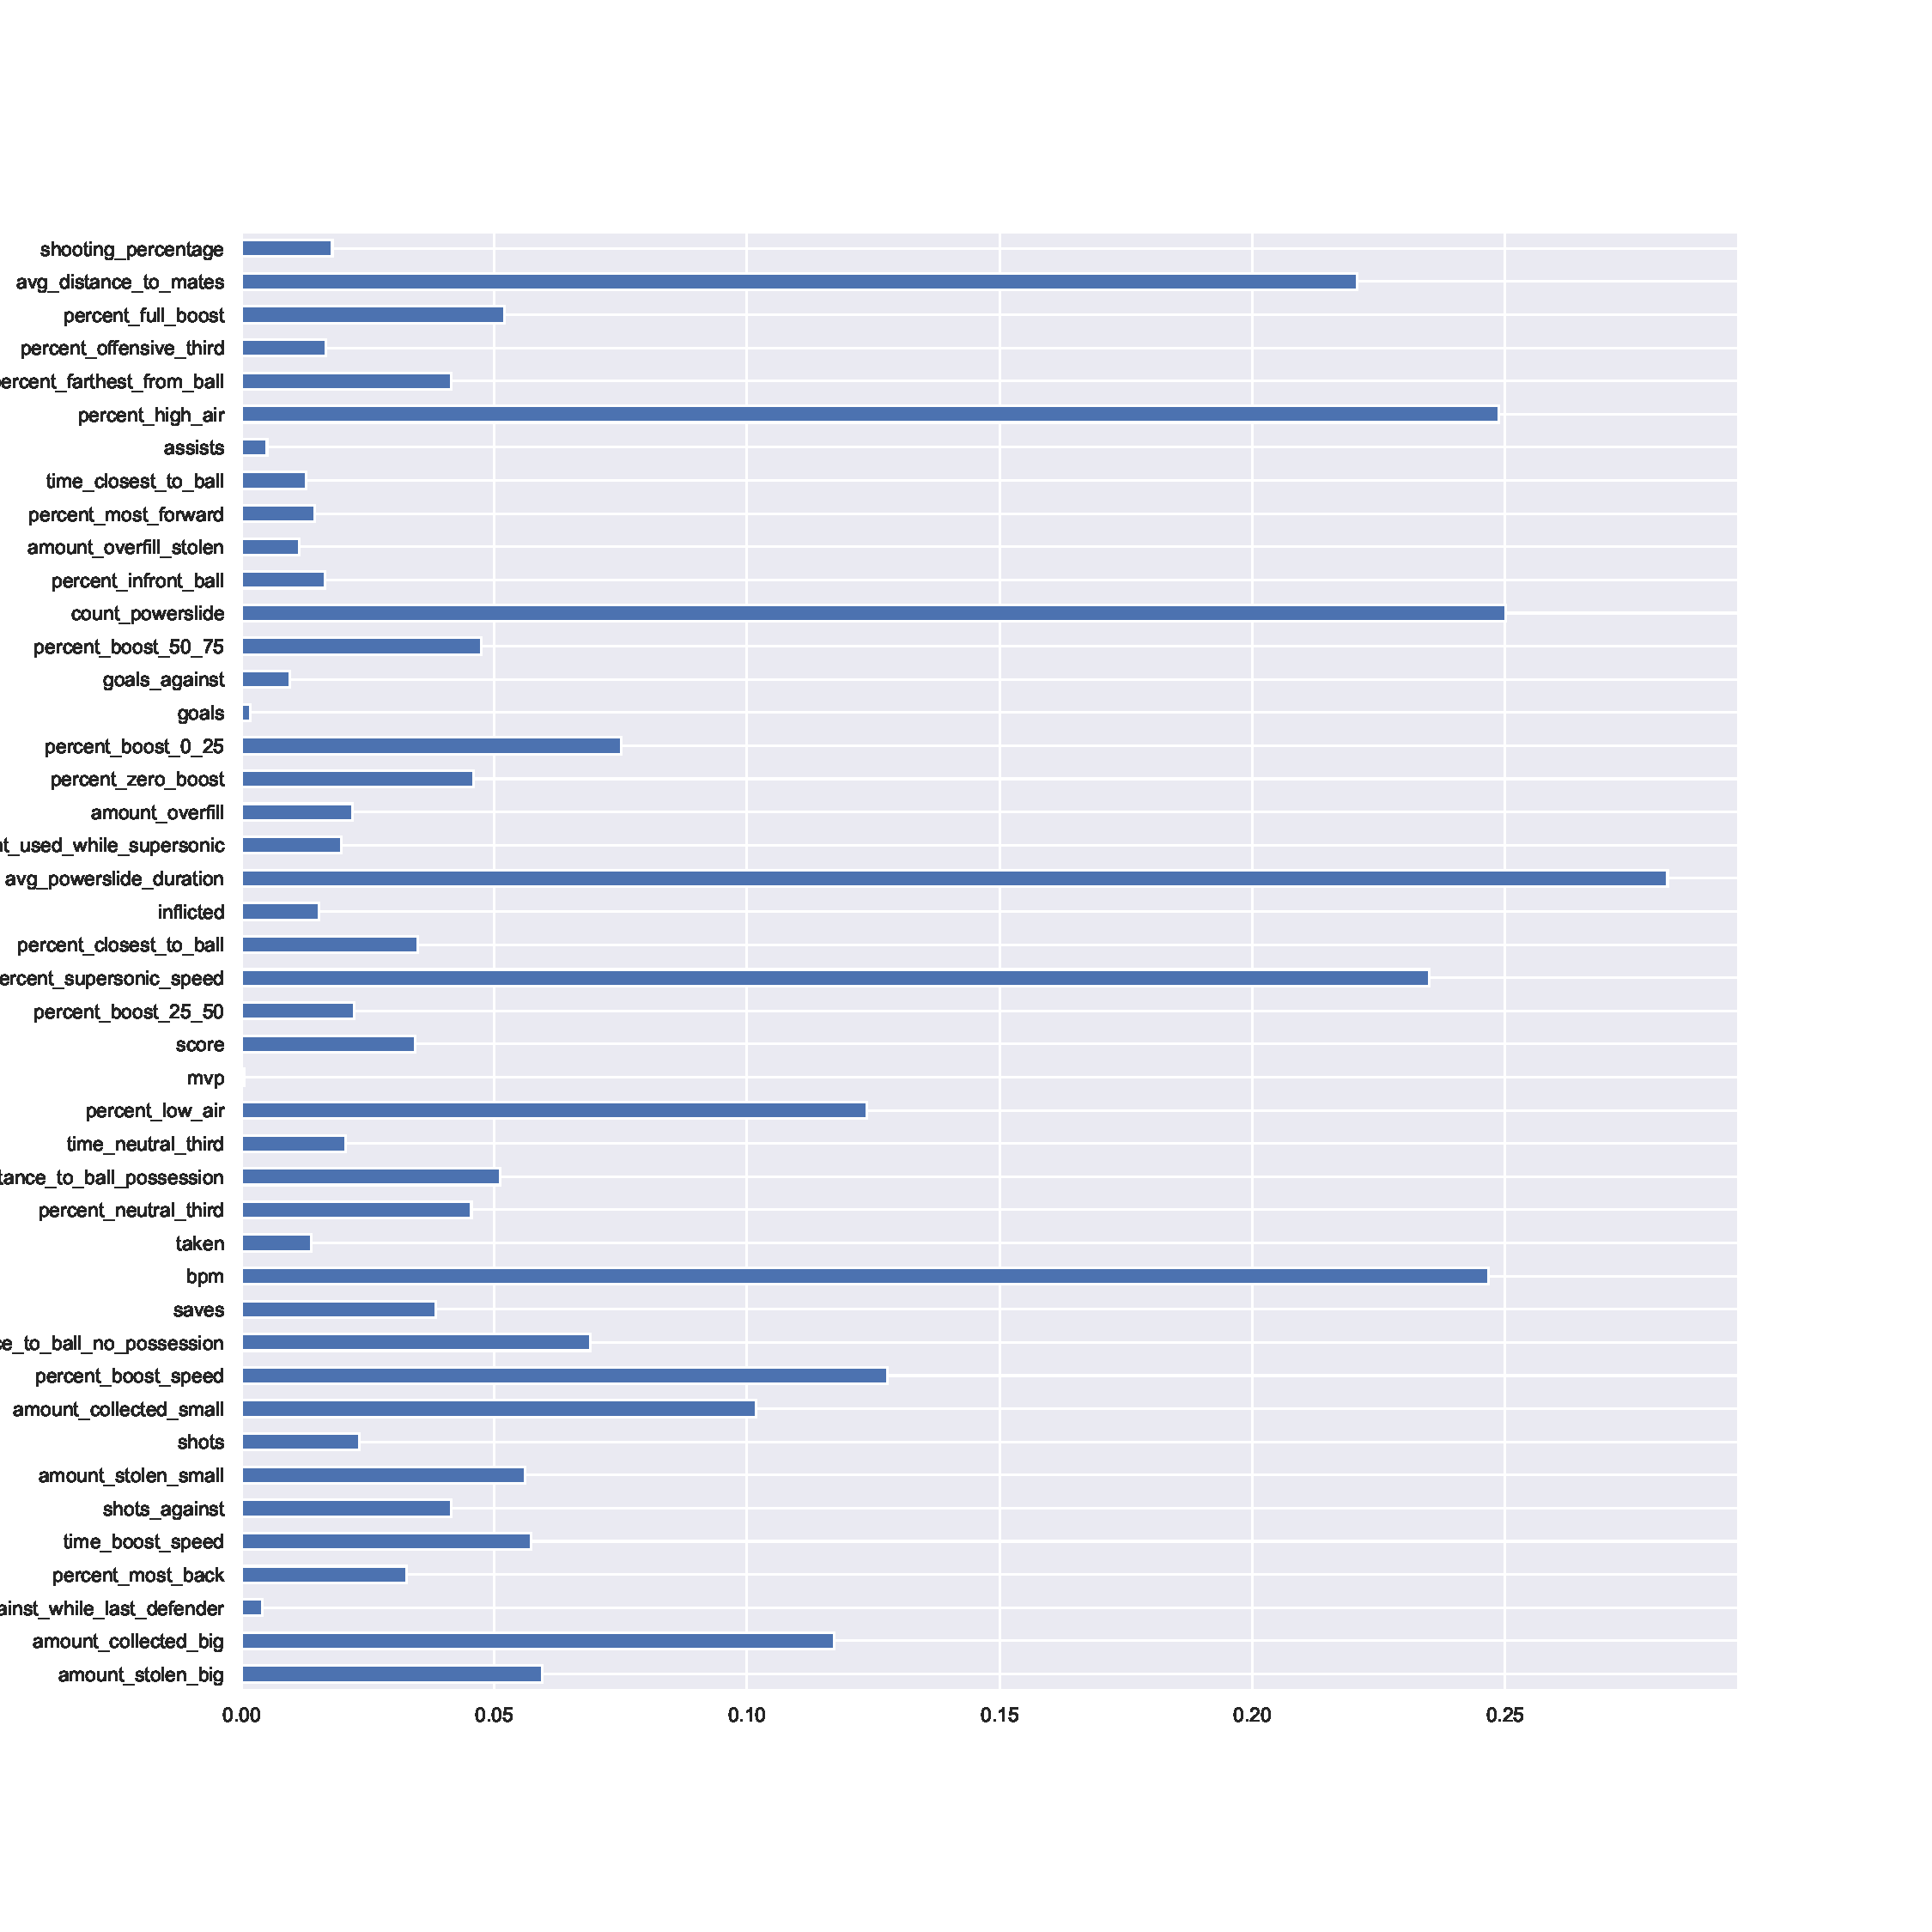
\includegraphics{res/imgs/ig.pdf}}
    \label{fig:ig}
    \caption{Information gain results}
\end{figure}

The results from thi test gave another insight on some kind of uninformative features. The features that are strictly related to the specific match and not on the playstyle and skill of the player. Such ones are \textit{goals}, \textit{mvp}, \textit{assists} and \textit{goals\_against\_while\_last\_defender} and have been removed. The final dataset counts 37 features.

\subsection{Data construction}

In this step there will be gonna built the final dataset provided to the models.

Features of this dataset have different measurement units and scales, therefore features with bigger scales will be considered more important for some models, for example linear regression. Data need to be scaled.
The used scaling technique is called \textit{Robust Scaling}, proper for skewed data. It subtract the median and divides using the \textit{interquantile range (IQR)} instead of the mean and the standard deviation differently from z-score. It has been used the IQR between the 1st quartile (25th quantile) and the 3rd quartile (75th quantile).
This procedure has been applied to all the features except for the percentages.
They range from 0 to 100, therefore they have been simply divided by 100 to make them range from 0 to 1 (\textit{Decimal scaling}). 

\subsubsection{Factor analysis}

Factor analysis is a linear statistical model. It is used to explain the variance among the observed variable and condense a set of the observed variable into the unobserved variable called factors. Observed variables are modeled as a linear combination of factors and error terms (Source). Factor or latent variable is associated with multiple observed variables, who have common patterns of responses. Each factor explains a particular amount of variance in the observed variables.
Factor Analysis addresses the problem of analyzing the structure of the interrelationships, among a large number of variables by defining a set of common underlying dimensions, known as \textbf{factors}. In this case, the analysis is suitable, and could improve the final metrics of the regressors.

Firstly, it is ran a statistical test, the \textbf{Bartlett test of Sphericity}; the result of the \textit{p-value} is 0.0, which is below the significance level, that is 0.01, this means that our data is suitable for PCA or factor analysis, in other terms, the correlation matrix is not an identity matrix, therefore there are variables that can be compressed because are correlated.
After that, it is performed another statistical test, the \textbf{Kaiser-Meyer-Olin} test. KMO estimates the proportion of variance among all the observed variables. Lower proportion is more suitable for factor analysis. KMO values range between 0 and 1. Value of KMO less than 0.6 is considered inadequate. The resulting value is 0.72, which is not excellent but still good to perform factor analysis.

The next step is choosing the number of factors, it is possible to use the Kaiser criterion or the scree plot.

\begin{lstlisting}[caption=Eigenvalues vector, label=lst:eig, numbers=none]
    6.66168999, 4.08644897, 2.83432441, 2.28558437, 1.84343317,
    1.7371591 , 1.68384878, 1.22659406, 1.0839006 , 0.9532351 ,
    0.93196593, 0.84942509, 0.81297165, 0.76319104, 0.71516273,
    0.69252737, 0.6741302 , 0.64726297, 0.62468648, 0.5875707 ,
    0.55865857, 0.47723509, 0.41265987, 0.36922481, 0.35178791,
    0.31810623, 0.31006858, 0.28431297, 0.24621891, 0.21714735,
    0.18559563, 0.15784588, 0.12932119, 0.12073377, 0.08820541,
    0.07776513
\end{lstlisting}

From \reflst{lst:eig}, it is possible to see that there are only 9 values above 1.

\begin{figure}[H]
    \resizebox{1.1\linewidth}{!}{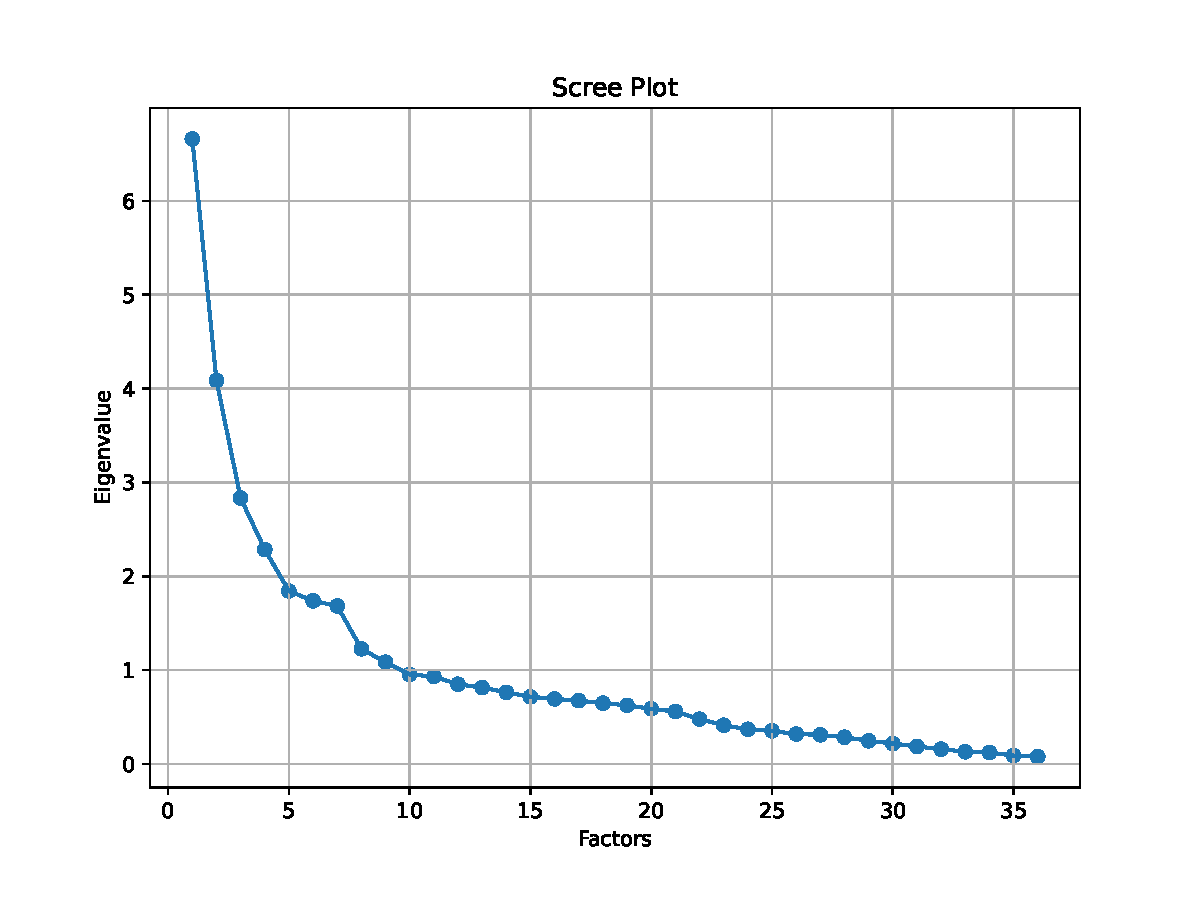
\includegraphics{res/imgs/scree.pdf}}
    \label{fig:scree}
    \caption{Scree plot} 
\end{figure}

Also from the scree plot \reffig{fig:scree}, the elbow is around 9-10, so it is possible to state that 10 factors should be adequate.
So the factor analysis is performed and \textit{factor loadings} are printed \reffig{fig:loadings}.

\begin{figure}[H]
    \resizebox{1.1\linewidth}{!}{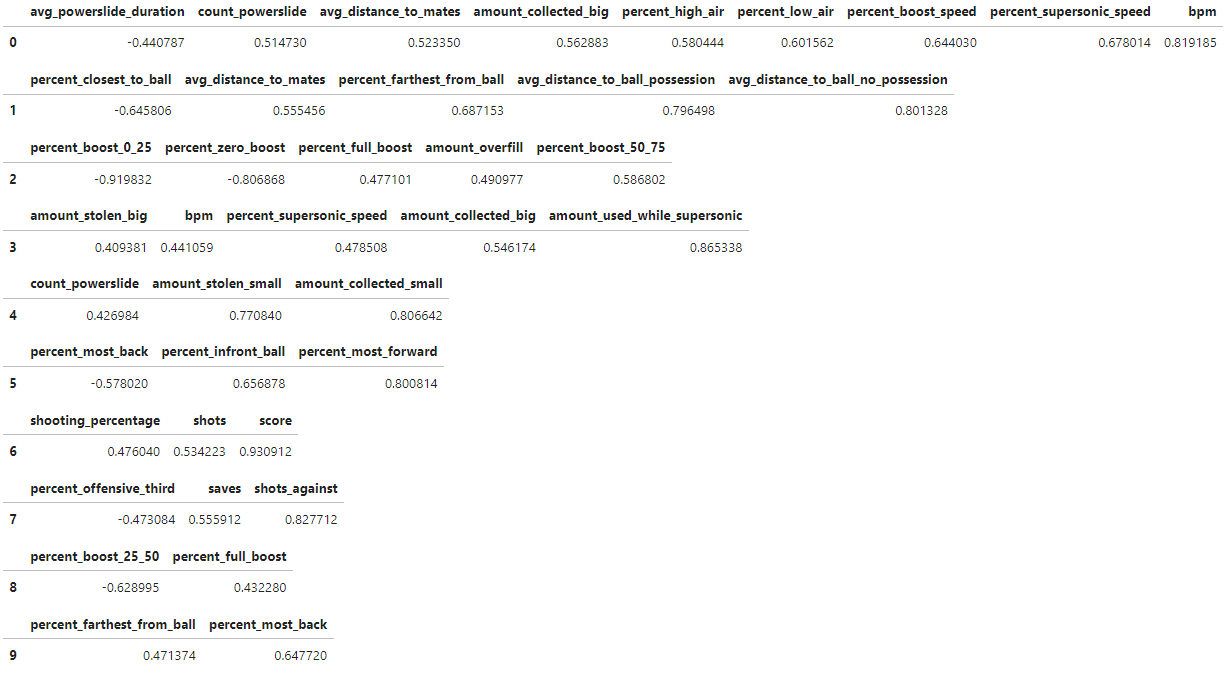
\includegraphics{res/imgs/loadings.png}}
    \label{fig:loadings}
    \caption{Loadings for each factor that are greater than 0.4 in absolute value} 
\end{figure}

Variables in factor 1, 5 and 9 are position related, those in factor 2 and 8 are all boost related, those in factor 3 are related to boost and speed. Factors 6 and 7 have some relations: about factor 6, shots give score and the amount of shots against is related with the number of saves; about factor 7, positioning in the field is related to the number of saves and shots received. Lastly, for factors 0 and 4 there are some related variables, but others doesn't have a clear interpretation of their relations.

\subsection{Format data}

Data is stored as a Comma Separated Values (CSV) file.

\subsection{Final produced datasets}

From the preparation phase we produced 5 datasets:

\begin{itemize}
    \item \textbf{Dataset preprocessed}: the dataset produced by the scaling;
    \item \textbf{Dataset factored}: the dataset produced by performing a factor analysis.
\end{itemize}